\section{Sensitivity Study}
A sensitivity study is done to get a better understanding of how different parameters of our contact tracing implementation affects the simulation. We have chosen to change the day we start the tracing, the quarantine period and the amount of traceable contacts. To see how these affect the effectiveness of contact tracing in the simulation. Only one variable will be changed at a time to ensure that we know exactly how a specific variable had an effect.
The base settings for our simulation is that the starting time for CT is set to 30 days, the number of contacts a person has each day is 10, the tracing of contacts goes 2 days back, the quarantine period for traced contacts is 14 days and the number of contacts that can be traced is a random number between 5 and 20. 

\subsection{Tracing start time}
Our standard start time for contact tracing we have set in our simulation is 30 days, in this section we will look at the effects it would have if it started earlier and later, for this we have tried to run the simulation with a start time of 15 and 60 days respectively. In the next couple of graphs we will see how this has an effect on the number of infected as well as the number of people put in quarantine.

\begin{figure}[H]
\centering
\begin{subfigure}{.5\textwidth}
  \centering
  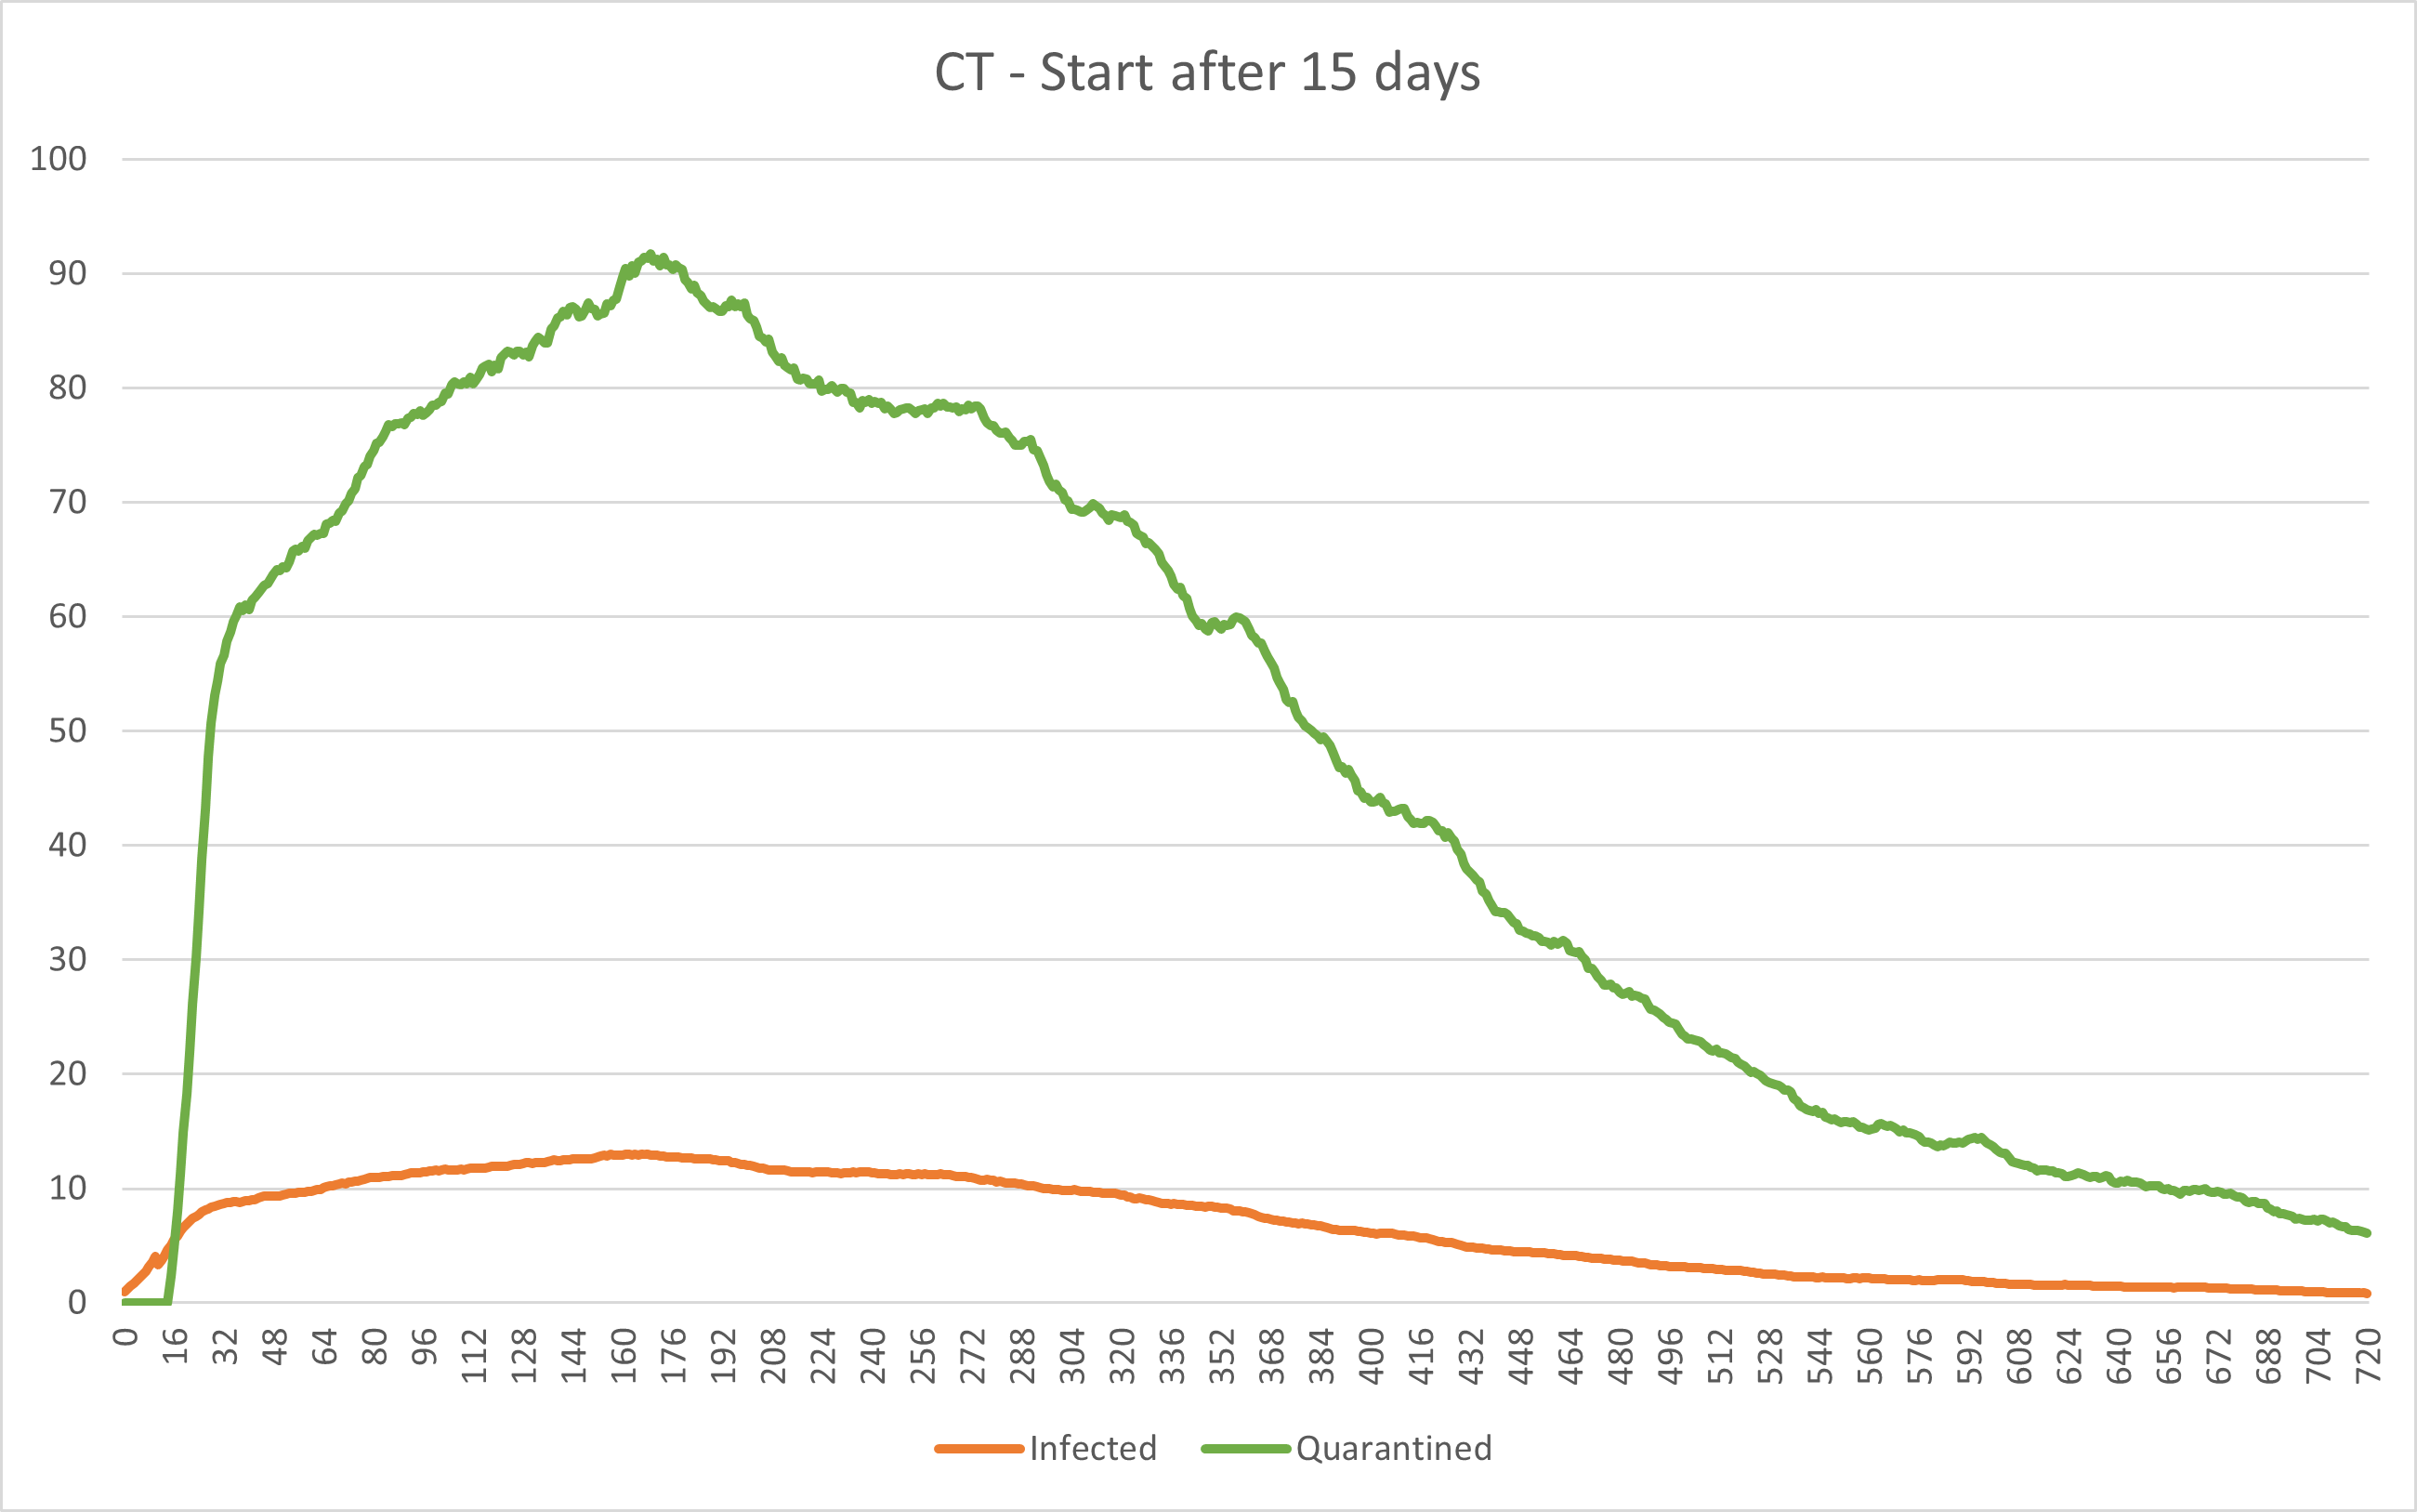
\includegraphics[width=.95\linewidth]{0_billeder/CT15Days.png}
  \caption{Contact tracing starting after 15 days}
  \label{Subfig:CT15}
\end{subfigure}%
\begin{subfigure}{.5\textwidth}
  \centering
  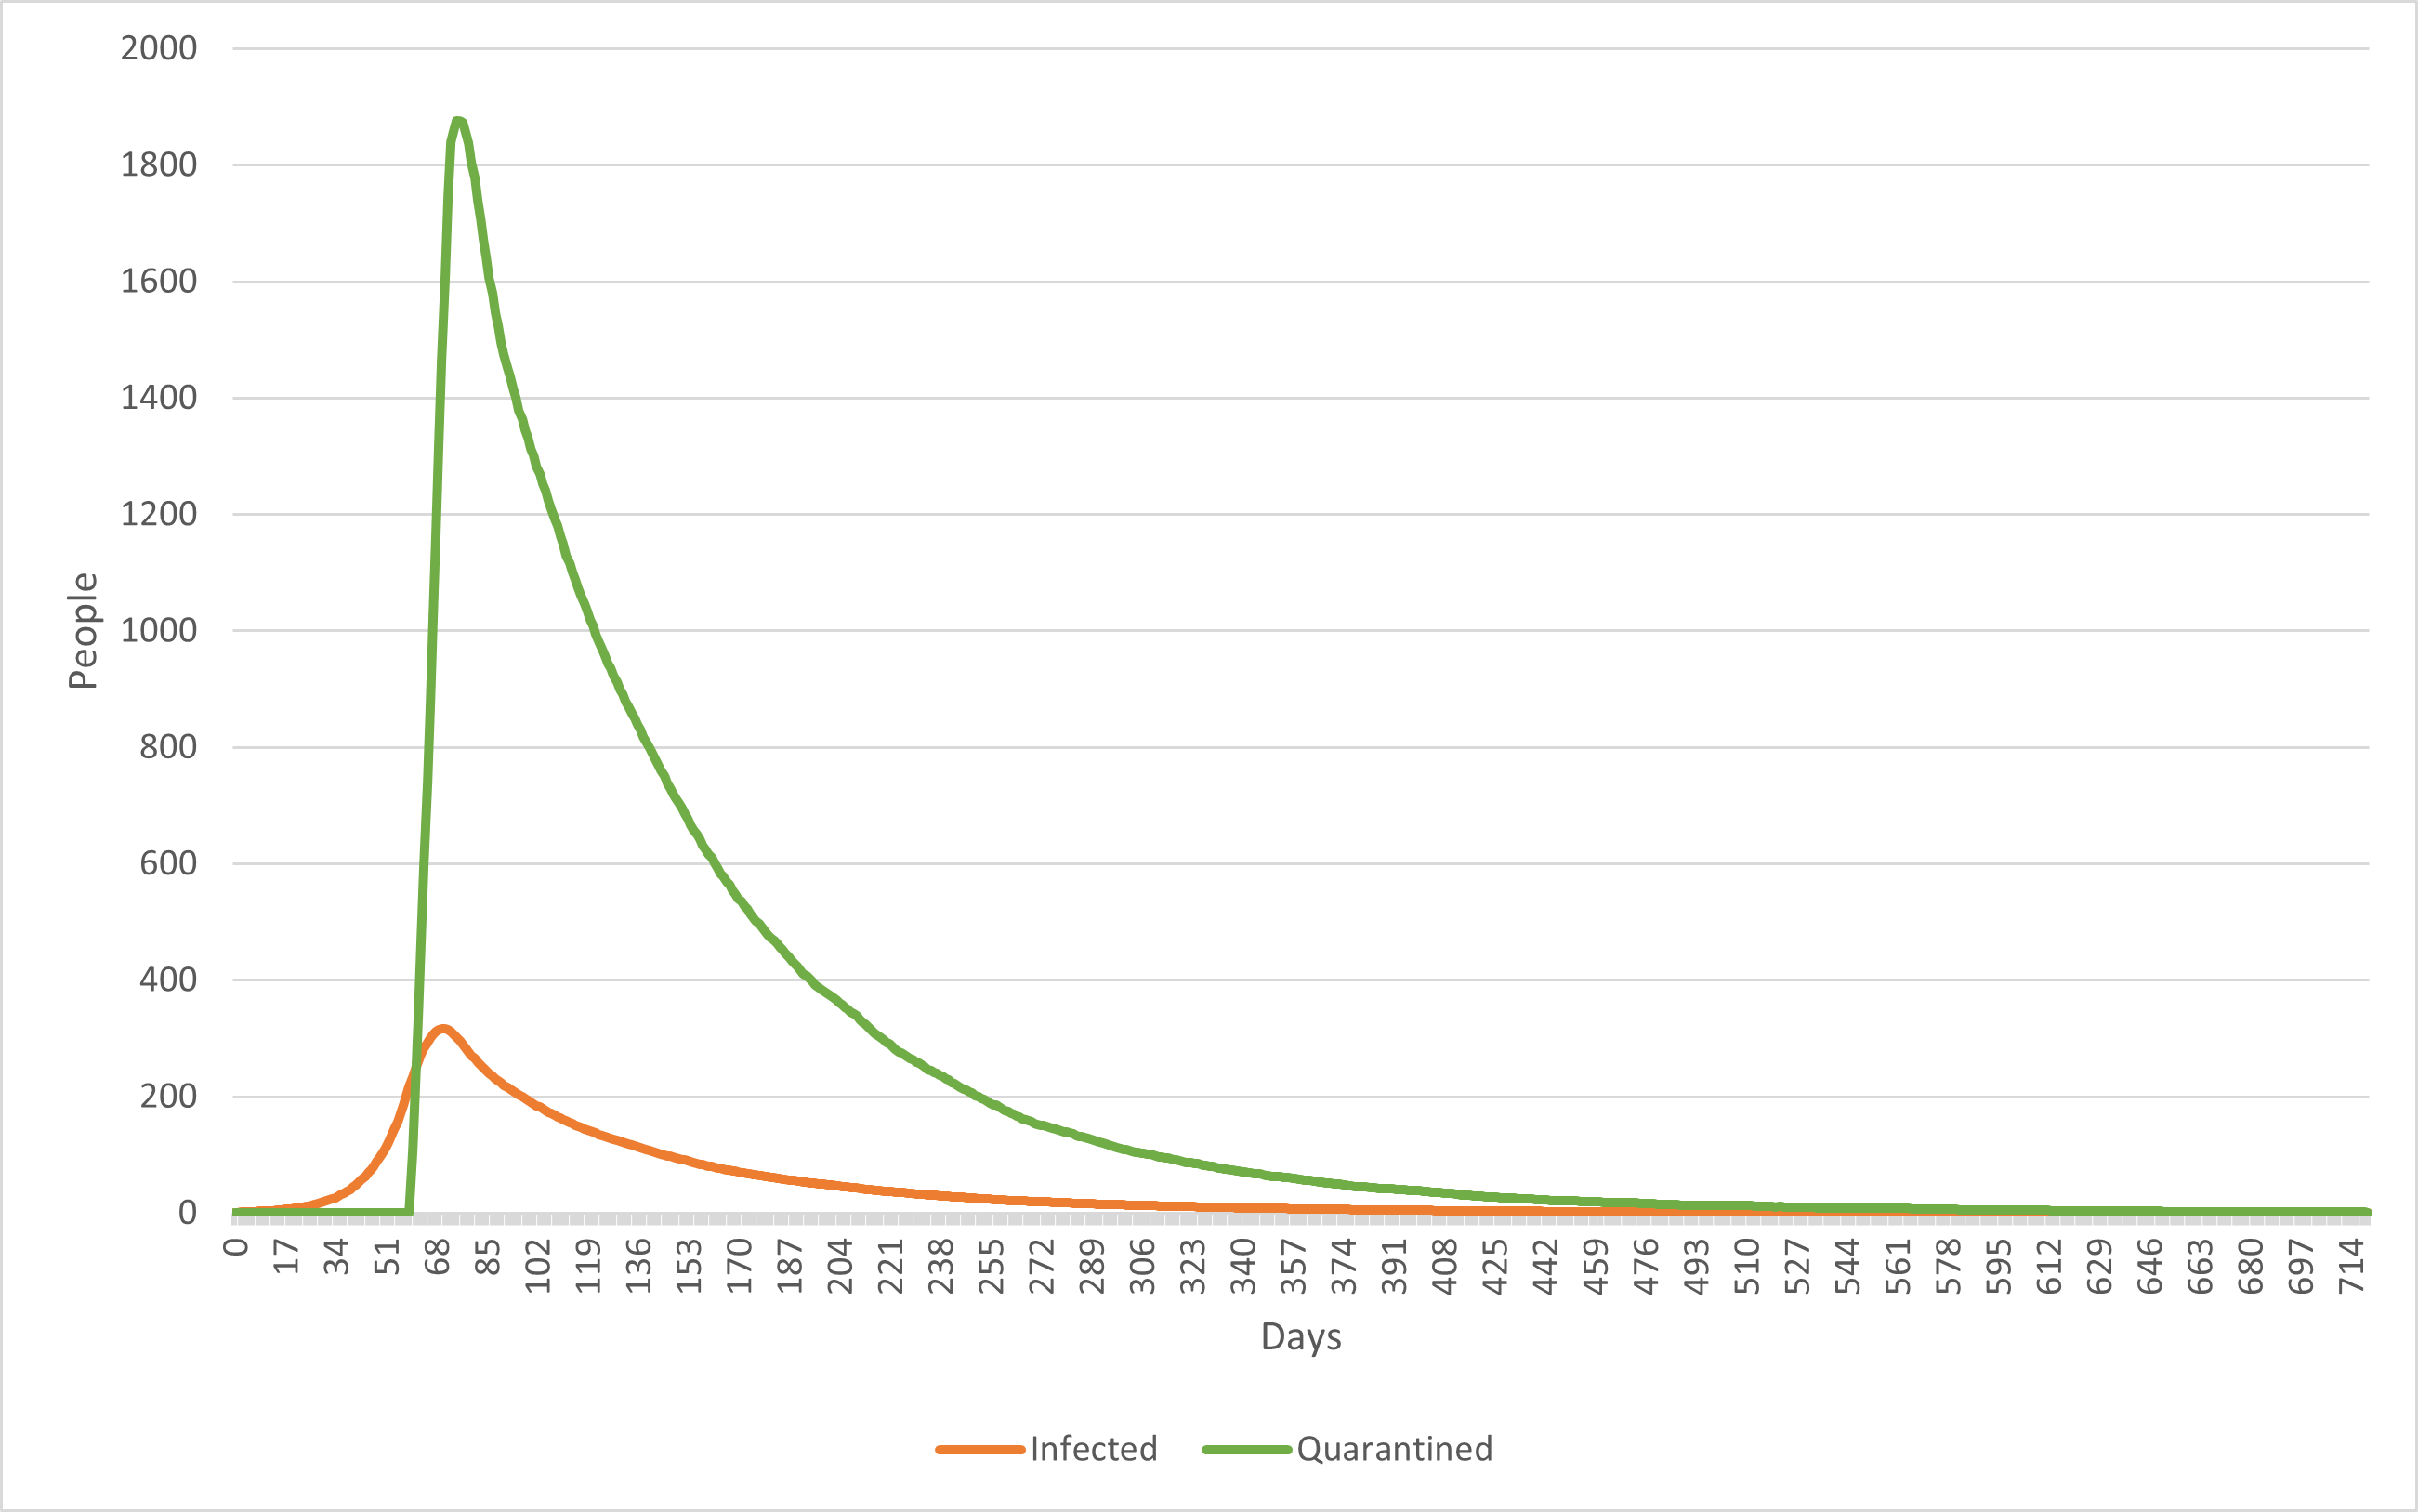
\includegraphics[width=.95\linewidth]{0_billeder/CT60Days.png}
  \caption{Contact tracing starting after 60 days}
  \label{Subfig:CT60}
\end{subfigure}
\caption{Graphs for number of people quarantined and infected plottet against days (Be aware of different proportions on the y-axis)}
\label{fig:CTstart1}
\end{figure}
From these graphs on figure \ref{fig:CTstart1} it can be seen that when we start tracing contacts in the population has a huge impact on both how many contacts that needs to be traced in total, as well as how many people become infected. It should also be noted that our simulation uses a much more \say{perfect} form of contact tracing, where everybody is at least able to trace 5 of their contacts over the previous 2 days. This is also the reason we see such a huge spike in the number of people quarantined when we reach the start time, since somewhere between 5-20 times the number of infected who are not asymptomatic and not in incubation will be quarantined.

It is also interesting to see that the early start in figure \ref{Subfig:CT15} results in a much more steady number of infected and a slow decline when its compared to the much later start on CT in figure \ref{Subfig:CT60}. This indicates that the earlier we start contact tracing the lower the amount of people who get infected and a substantial lower amount of the population needs to be traced.

\begin{figure}[H]
\centering
\begin{subfigure}{.5\textwidth}
  \centering
  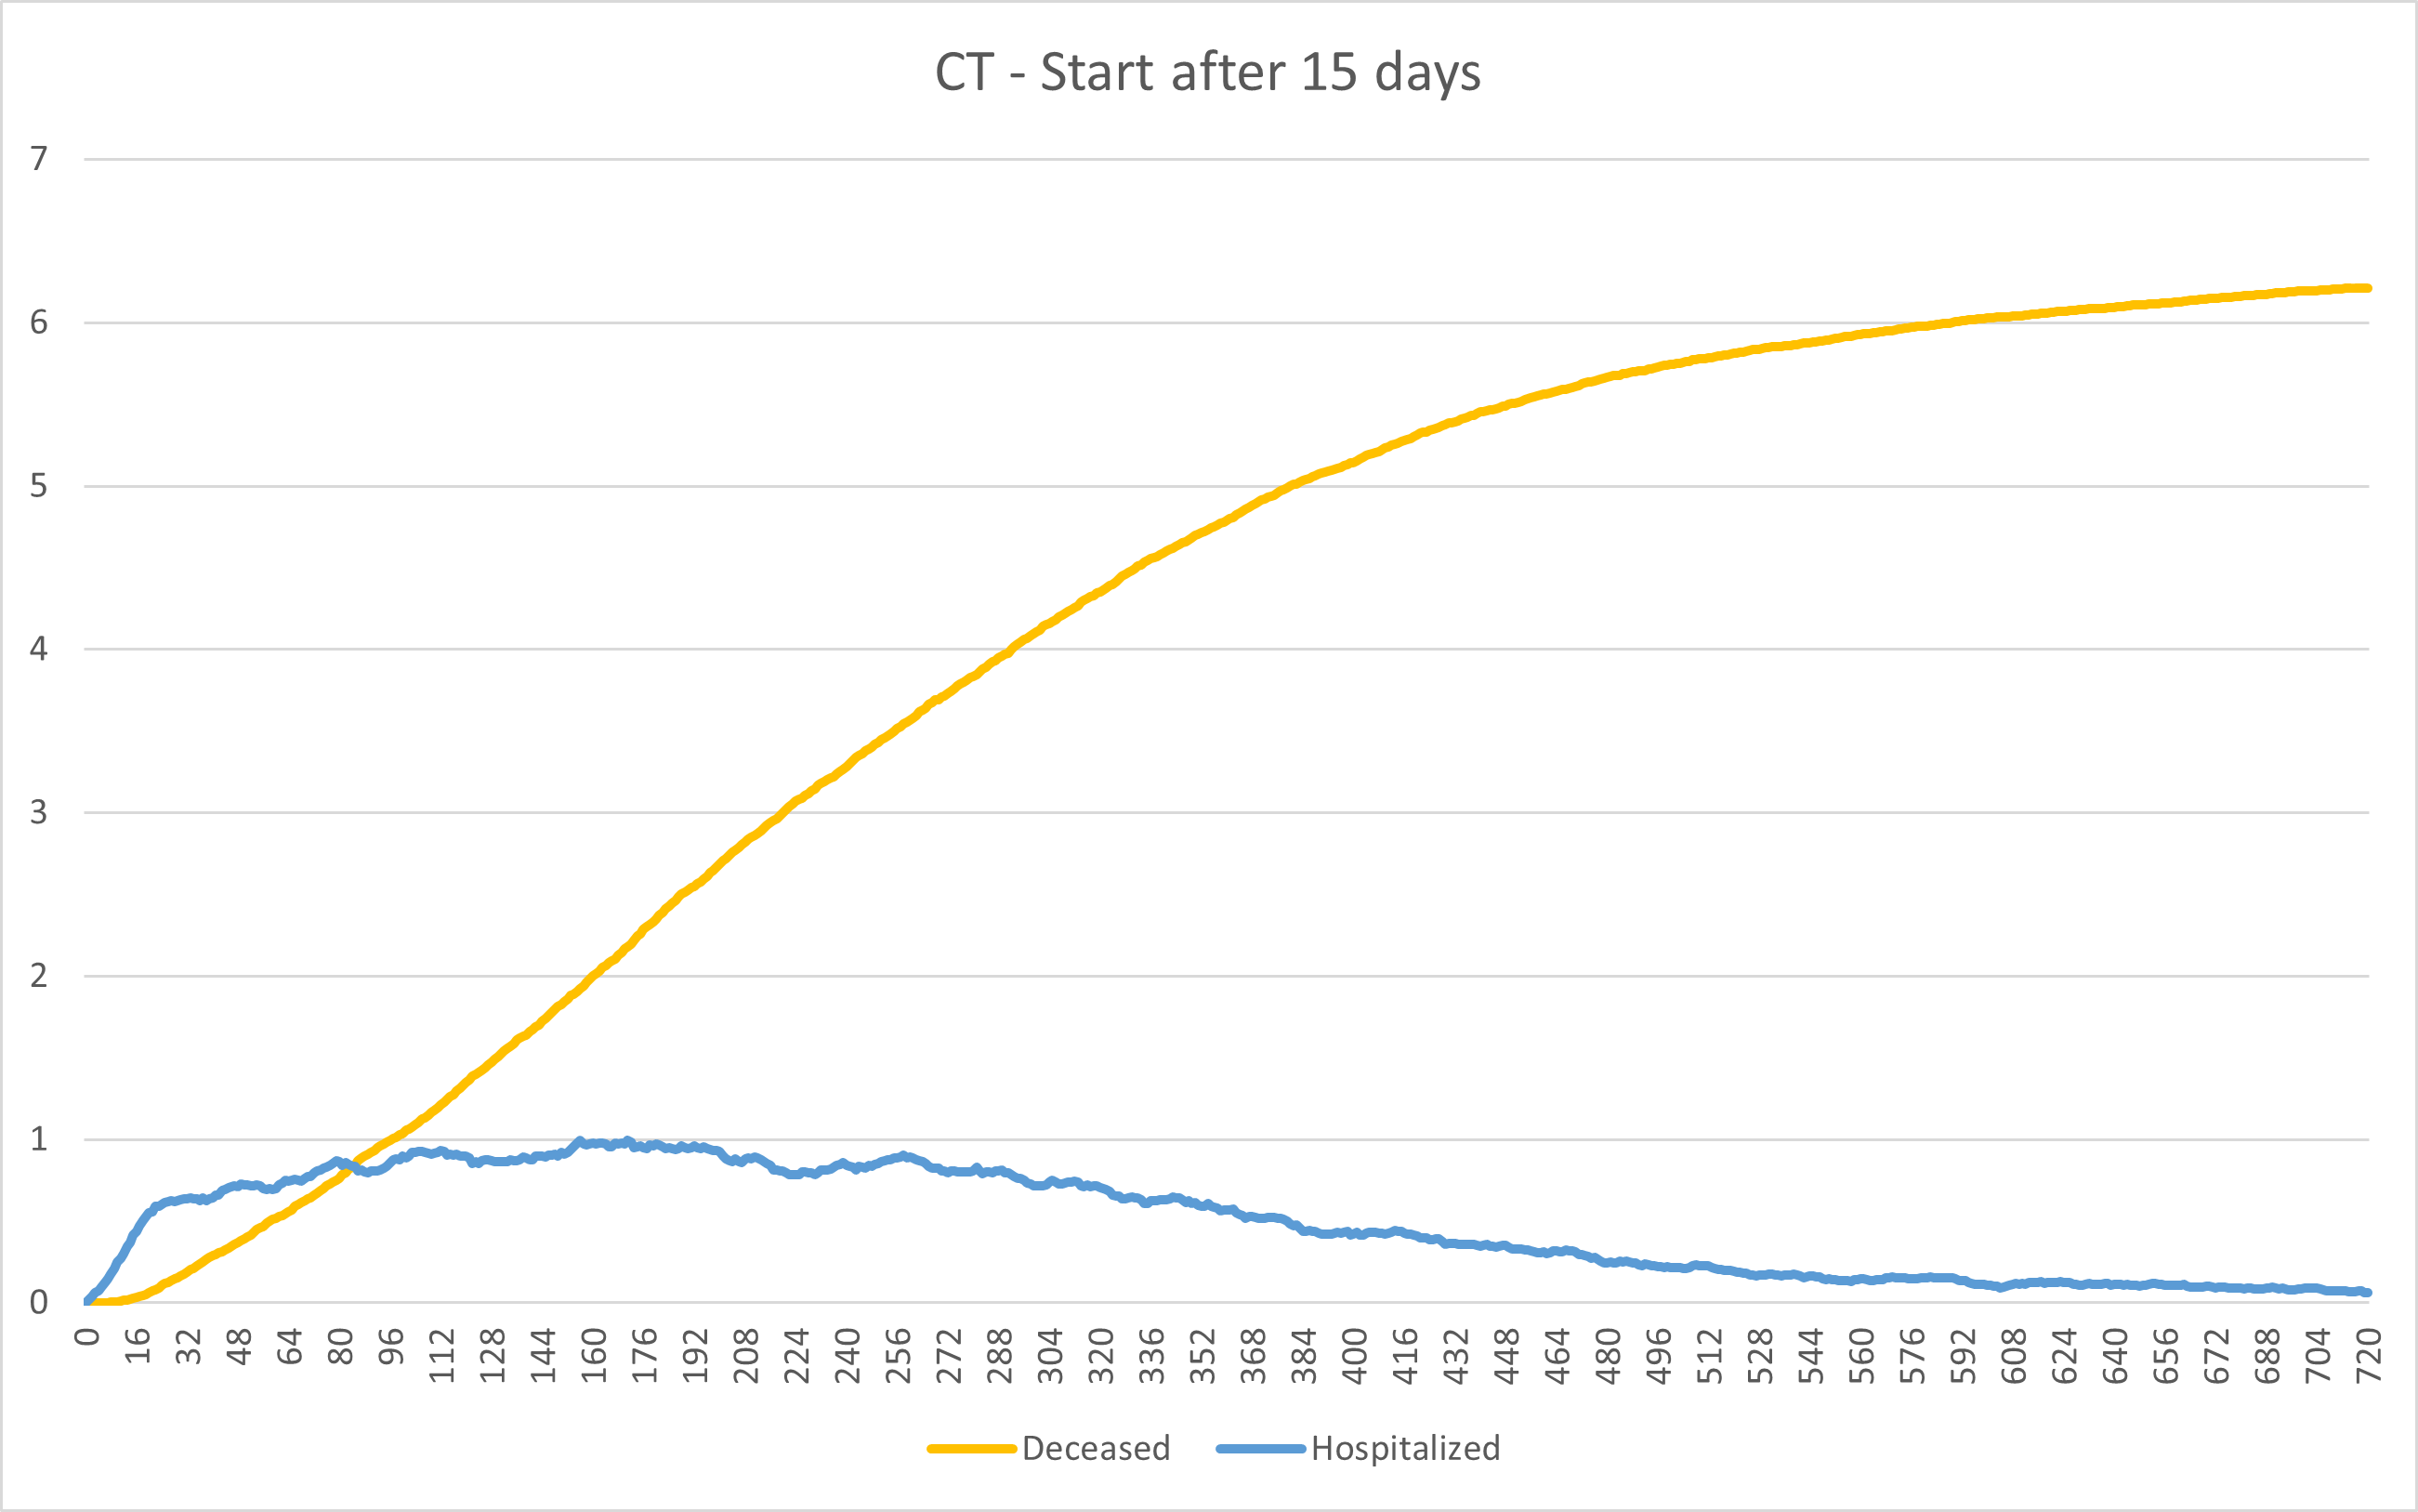
\includegraphics[width=.95\linewidth]{0_billeder/CT15DaysDH.png}
  \caption{Contact tracing starting after 15 days}
  \label{Subfig:CT15DH}
\end{subfigure}%
\begin{subfigure}{.5\textwidth}
  \centering
  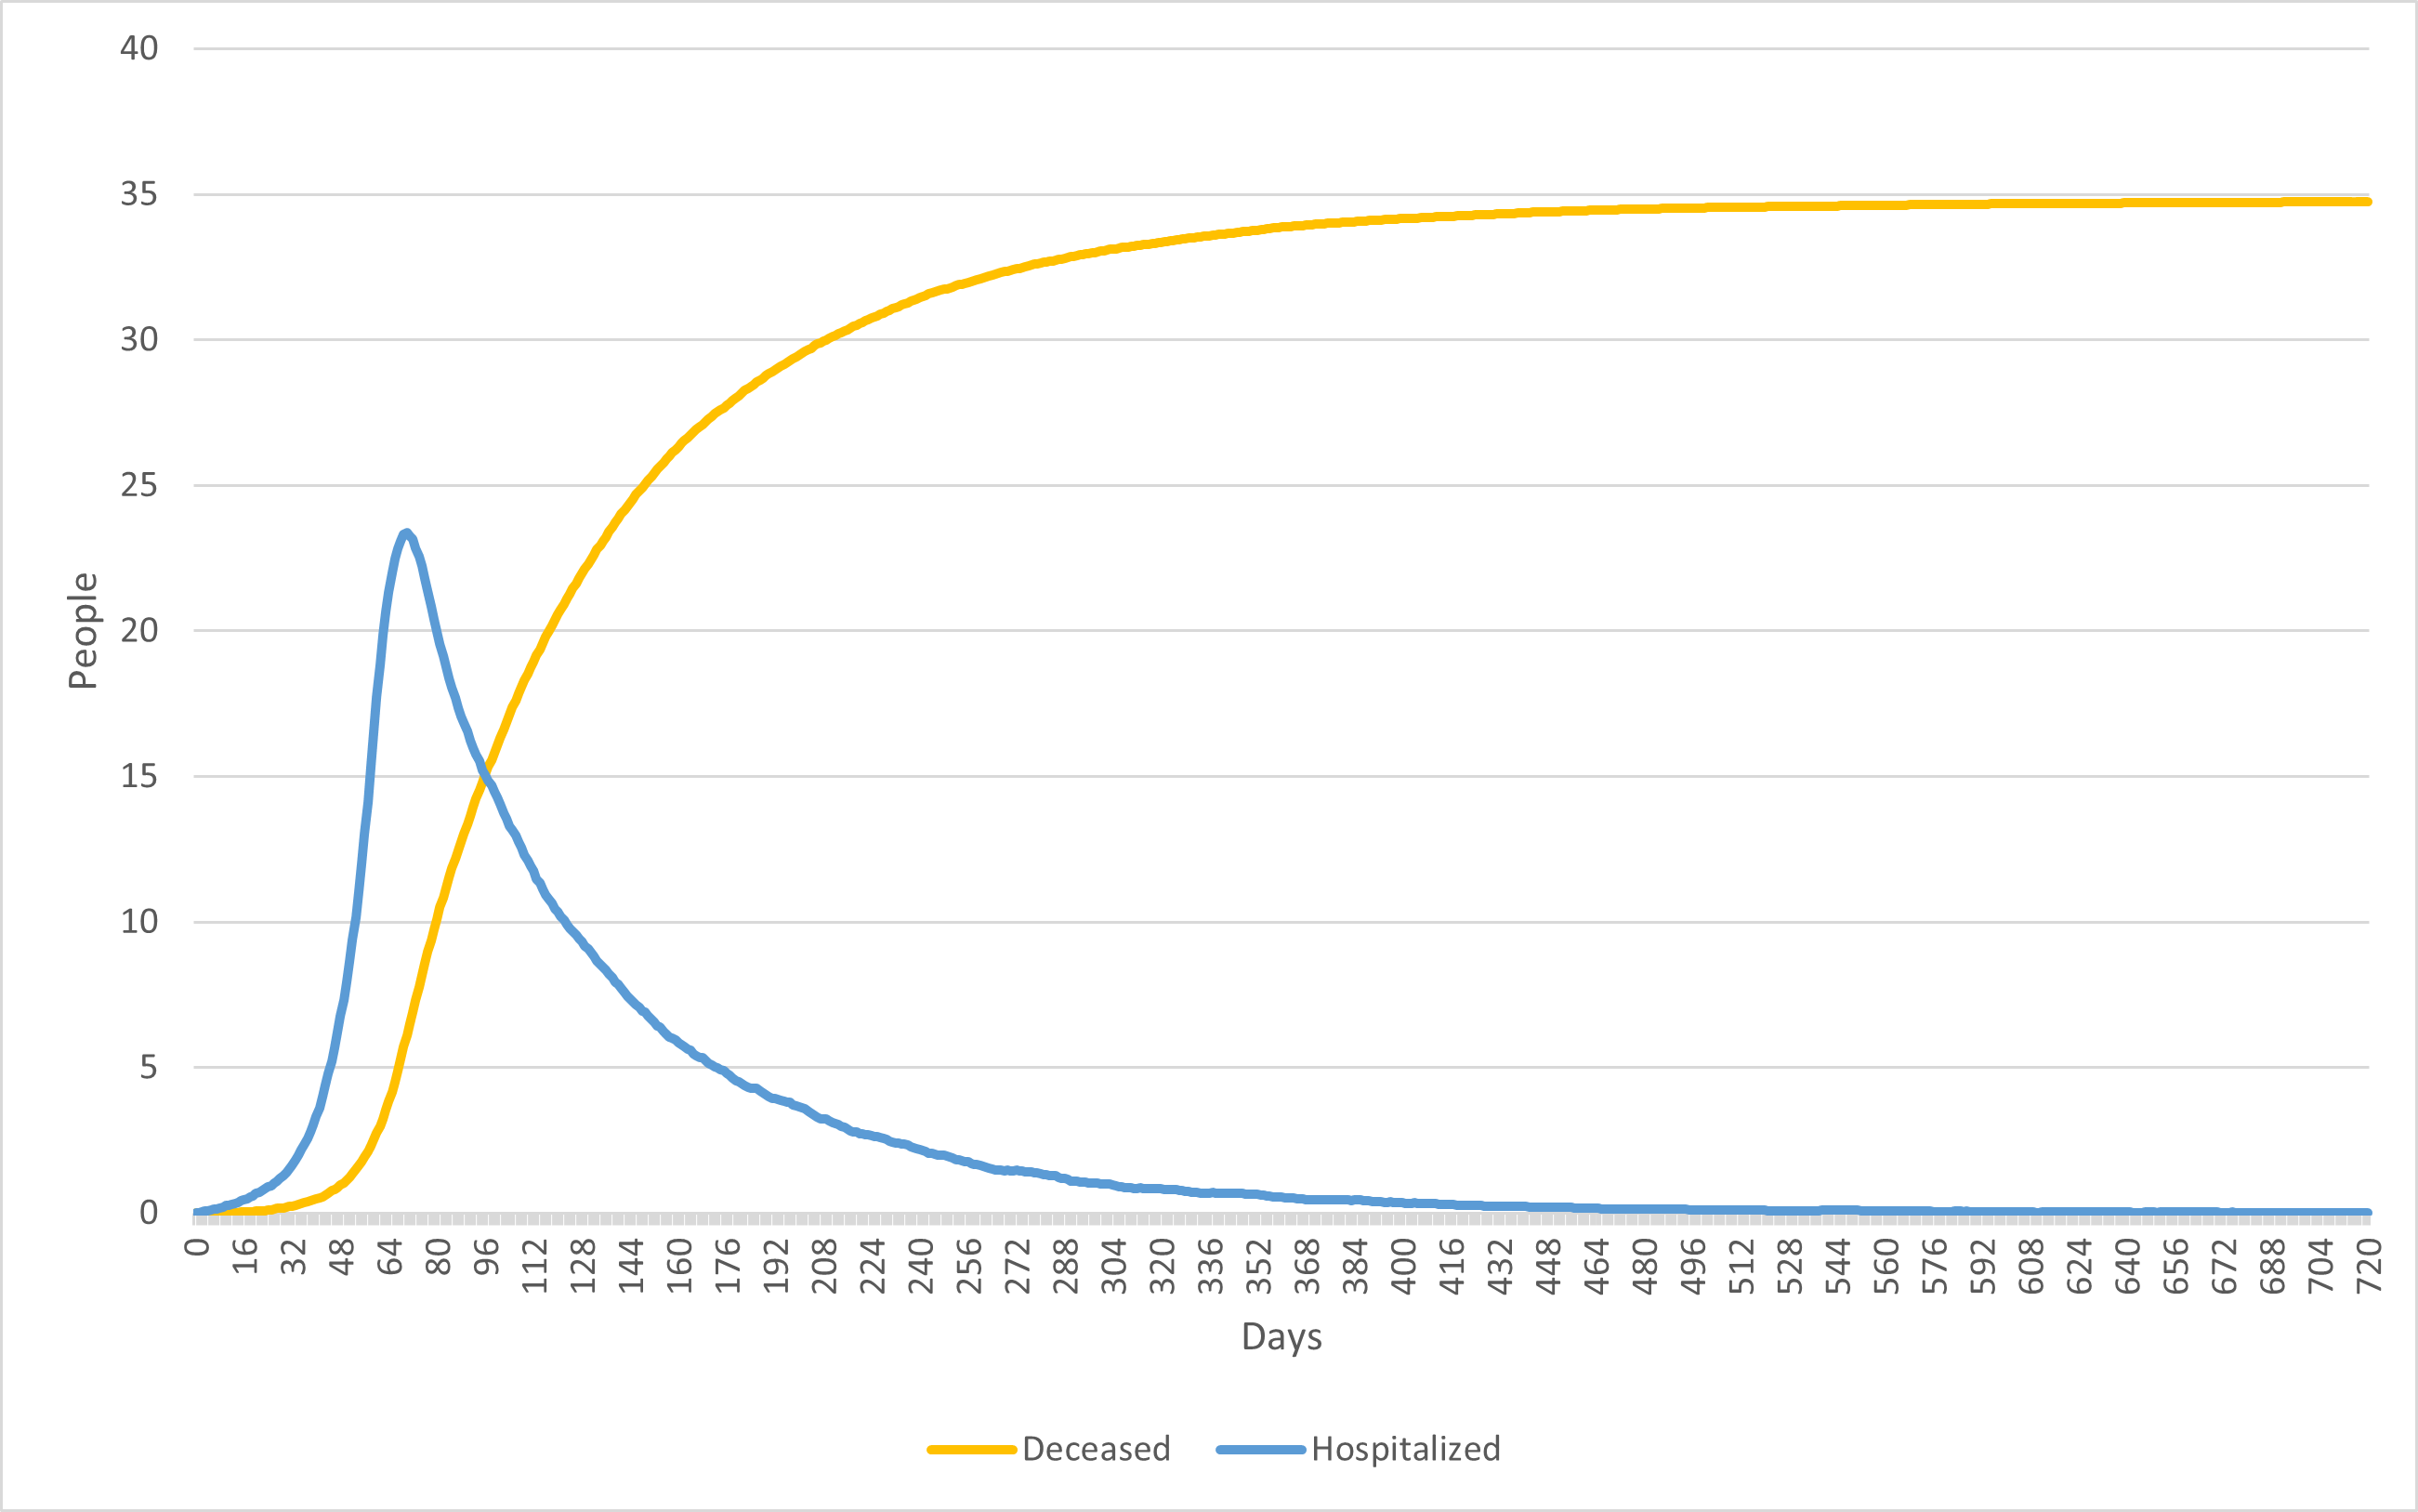
\includegraphics[width=.95\linewidth]{0_billeder/CT60DaysDH.png}
  \caption{Contact tracing starting after 60 days}
  \label{Subfig:CT60DH}
\end{subfigure}
\caption{Graphs for number of people hospitalized and deceased plottet against days (Be aware of different proportions on the y-axis)}
\label{fig:CTstart2}
\end{figure}

Since the starting time had such a notable effect on the number of people who became infected, it also had 


\subsection{Quarantine Period}
In this section we are looking at how the quarantine period will affect the amount of persons getting infected. We have run a simulation with a quarantine period of 7 day and one with 21 days. The two graphs below show how the two quarantine periods affect the amount people getting infected and are put into quarantine.


\begin{figure}[H]
\centering
\begin{subfigure}{.5\textwidth}
  \centering
  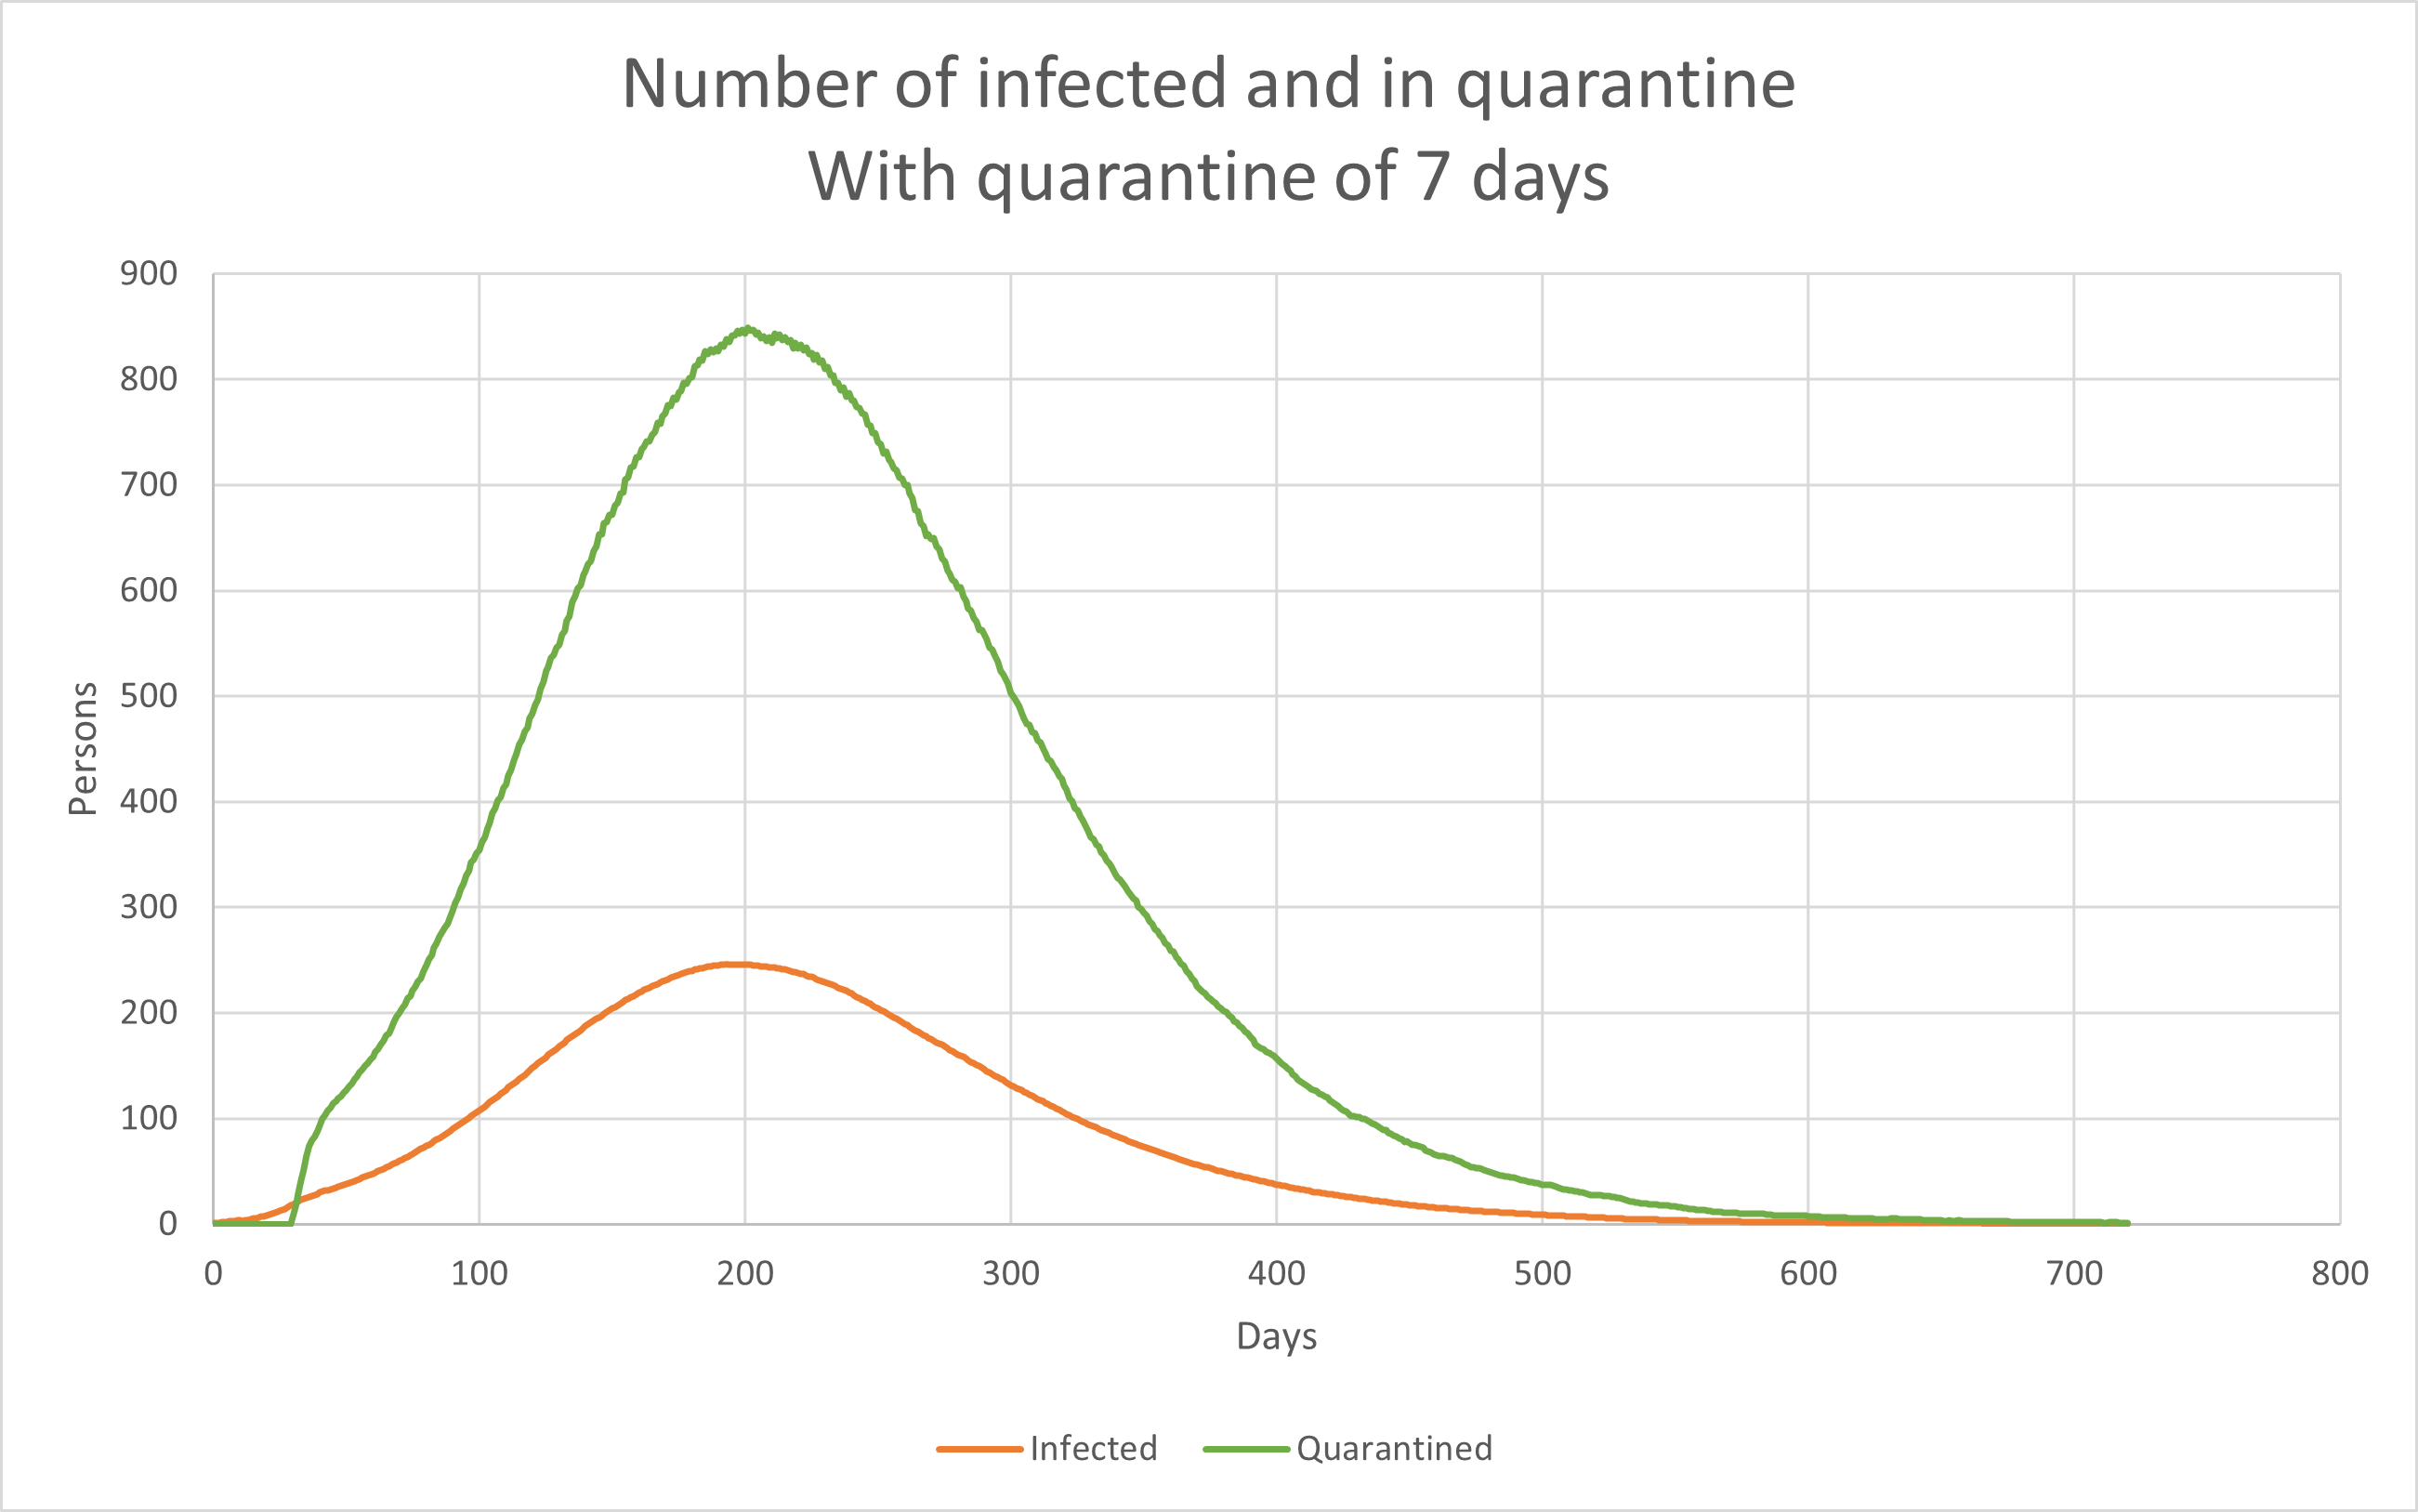
\includegraphics[width=.95\linewidth]{0_billeder/CT_Q_7.png}
  \caption{Quarantine period of 7 days}
  \label{fig:sub1}
\end{subfigure}%
\begin{subfigure}{.5\textwidth}
  \centering
  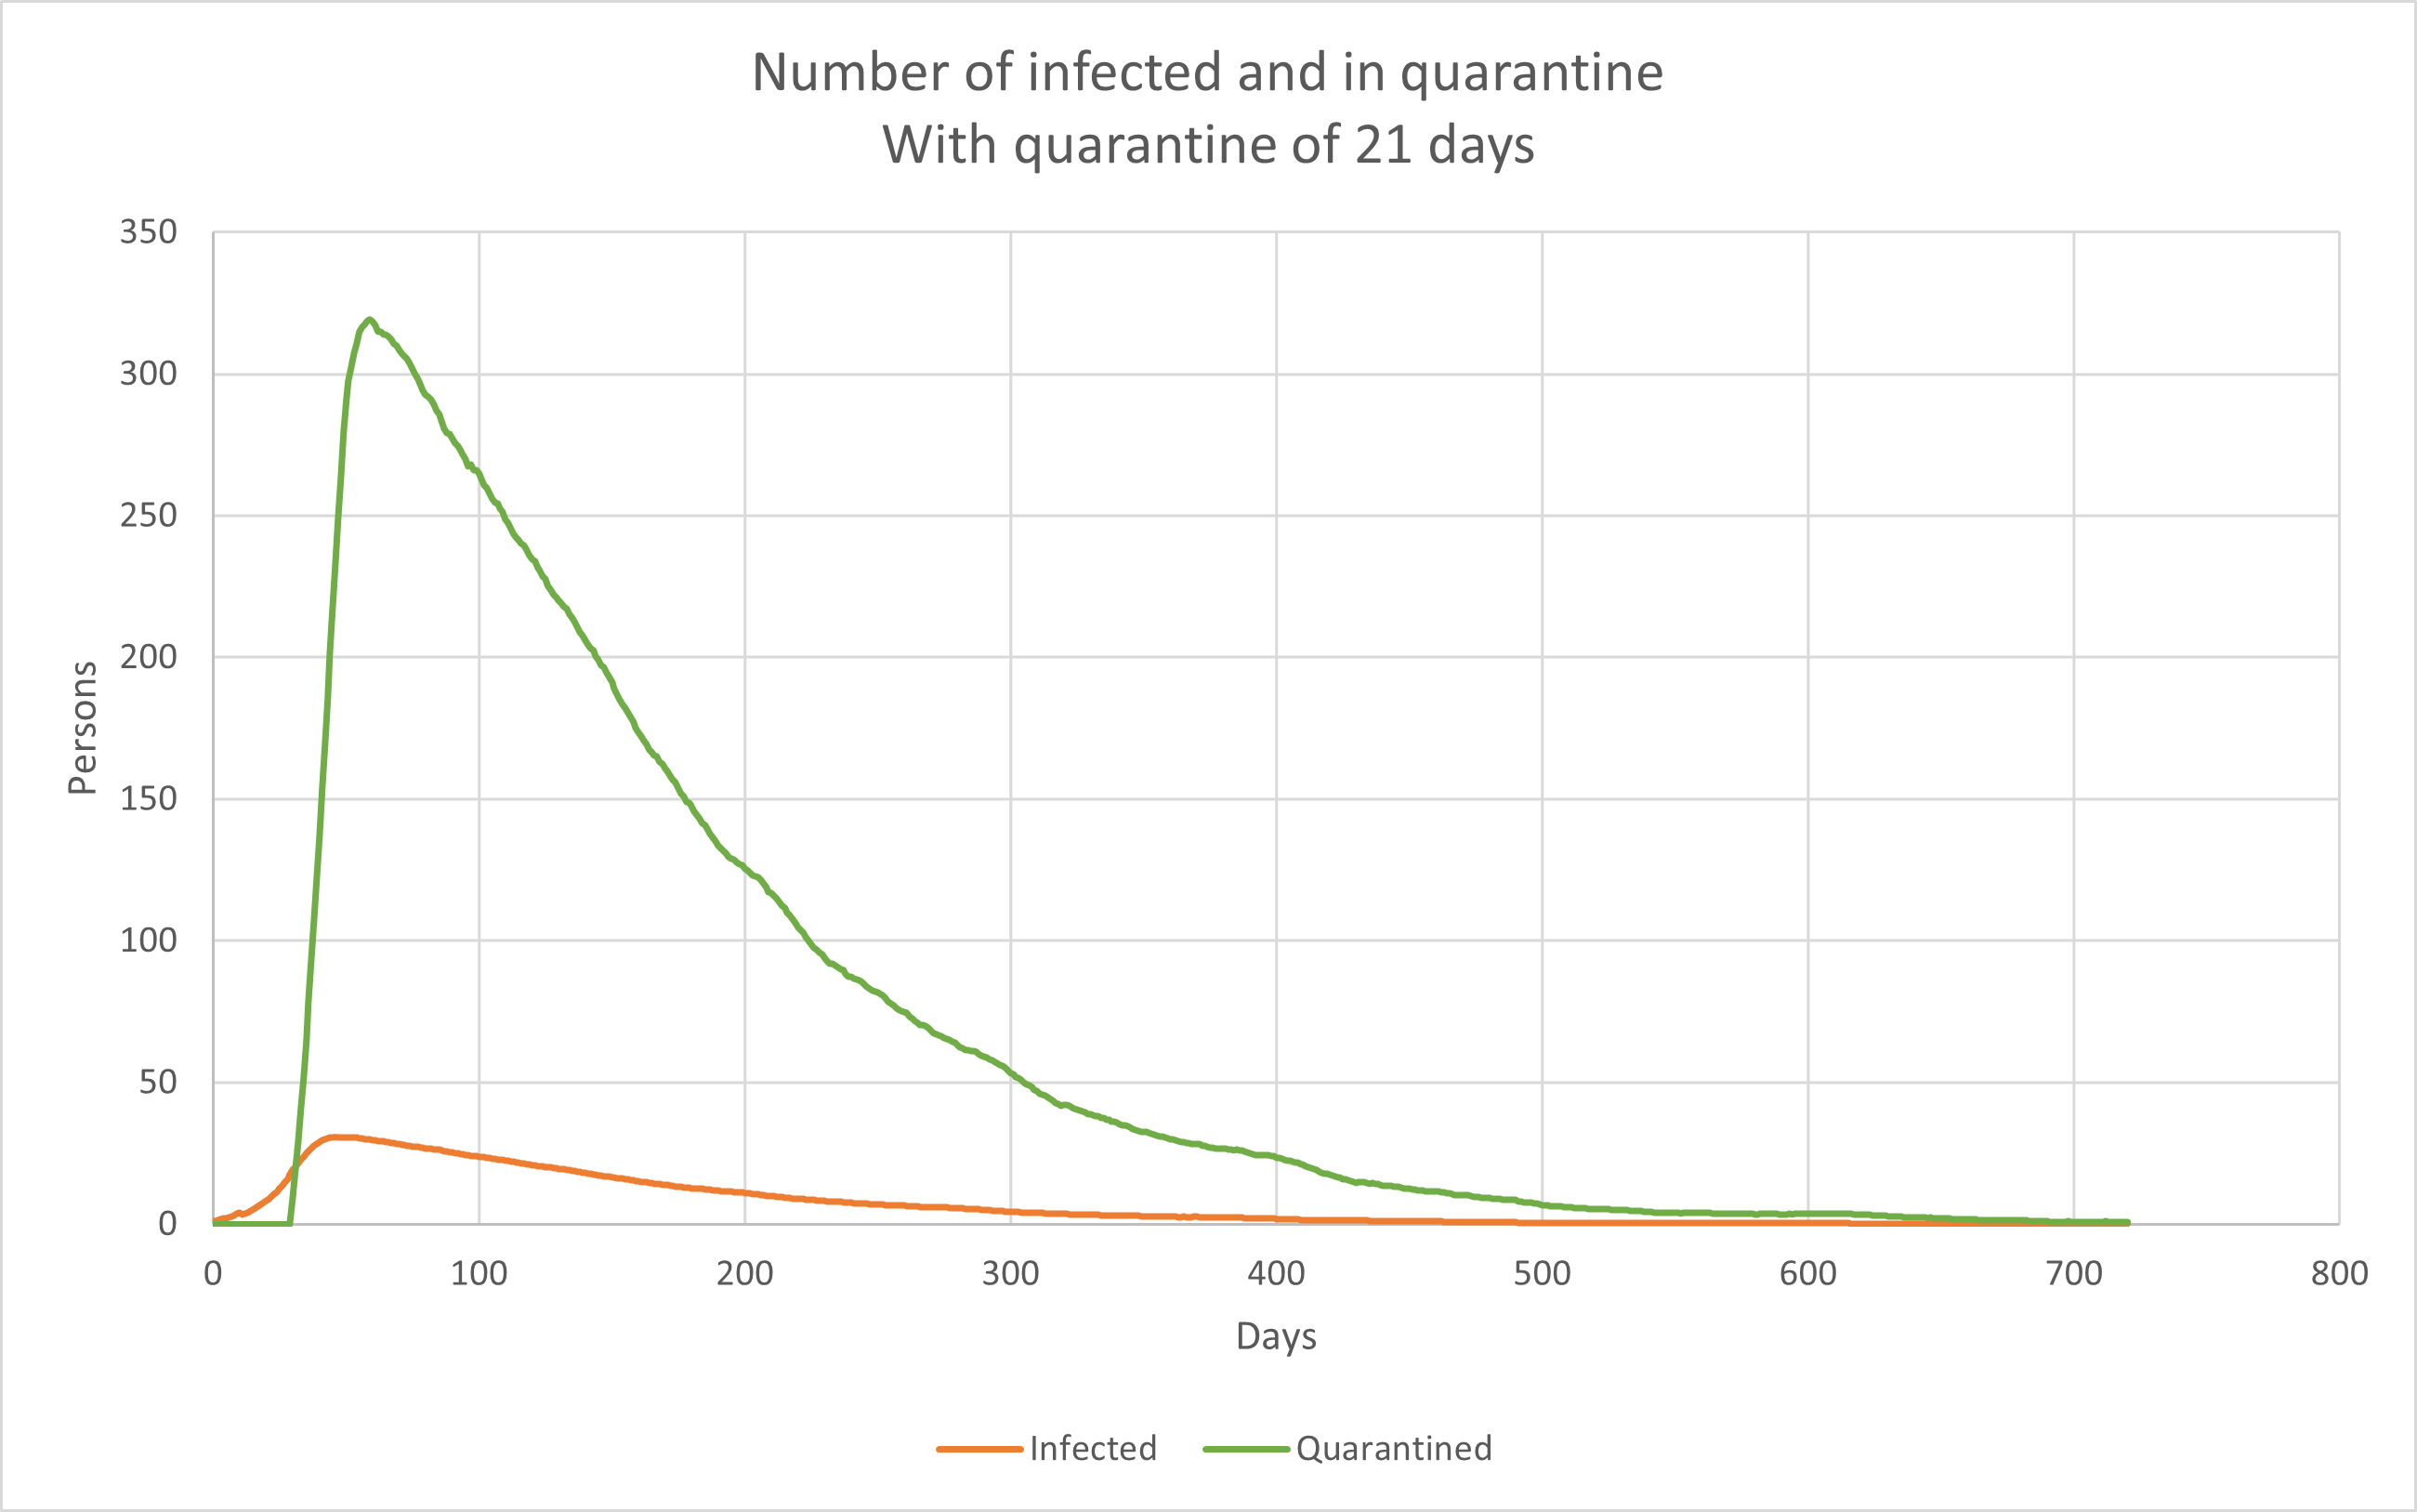
\includegraphics[width=.95\linewidth]{0_billeder/CT_Q_21.png}
  \caption{Quarantine period of 21 days}
  \label{fig:sub2}
\end{subfigure}
\caption{Comparison between 7 day and 21 day quarantine period}
\label{fig:test}
\end{figure}

The graphs show that when the quarantine period is increased, we see that we have a much lower 

\subsection{Traceable contacts}

